%!TEX root = ../thesis.tex
\chapter{Fundamentals}
\label{ch:fundamentals}

\section{Computer Vision}
Computer vision is a subfield of artificial intelligence that is closely linked to image processing and machine learning. It extends raw data acquisition with methods that combine digital image processing, pattern recognition, machine learning and computer graphics. The aim is to give machines the human ability to extract and interpret information from images \citep{Wiley2018}. Algorithms and optical sensors are used to obtain information and simulate human visual perception \citep{Matiacevich2013}. A distinction can be made between image acquisition and image analysis. Important components of image analysis include:
\begin{itemize}
    \item \textbf{Image generation:} Saving an object as a digital image.
    \item \textbf{Image processing:} Improving image quality to increase information content.
    \item \textbf{Image segmentation:} Separating the object from the background.

    \item \textbf{Image measurement:} Determination of significant image points (so-called features).
    \item \textbf{Image interpretation:} Derivation of semantic information from the image data \citep{Mery2013}.
\end{itemize}





\section{Machine and Deep Learning}
Machine learning describes an approach in computer science in which algorithms independently recognise patterns based on existing data in order to achieve a defined goal – such as the classification of information. In contrast to traditional algorithms, which follow fixed rules specified by humans, a learning algorithm develops its own processing strategies. The decision logic is not created through manual programming, but through the analysis of data and the recognition of recurring structures \cite{Shetty2022}. The term ‘learning’ generally refers to the process of acquiring knowledge or skills through experience, trial and error, instruction or observation. Applied to the machine context, this means that machines are able to generalise from examples and process new, unknown data through repeated analysis and feedback. Machine learning can therefore be understood as a computer-assisted replication of human learning processes, in which algorithms are able to develop abstract rules from raw data and apply them to new situations \cite {Fischer1999, Braga-Neto2020}. This ability opens up new possibilities for solving complex problems that are difficult or impossible to tackle with conventional, rule-based methods \cite{Goodfellow-et-al-2016}.



\begin{figure}[h]
    \centering
    \includegraphics[width=0.6\textwidth, clip, trim= 2cm 8cm 2cm 2cm]{svg-inkscape/ML_and_DL_svg-tex.pdf}
    \caption{Overview over Artificial Intelligence, Machine Learning and Deep Learning. \cite{Alzubaidi2021}}
    \label{fig:ML_andD_L}
\end{figure}

\acrfull{DL} is a subfield of machine learning (see Fig. \ref{fig:ML_andD_L}) whose functionality is inspired by the neural processes in the human brain. It simulates the information processing that takes place in the central sensory regions of the brain. In contrast to classic rule-based methods, \acrshort{DL} does not work with rules strictly designed by humans, but uses large amounts of data to recognise patterns and analyse inputs for specific characteristics. A characteristic feature is the use of numerous layers \acrfullpl{ANN}, in which each layer interprets the supplied information in a unique form. While conventional machine learning techniques usually rely on a separation of pre-processing, feature extraction, feature selection, learning and classification, \acrshort{DL} can partially automate these steps and combine them into a single end-to-end process. This enables both the learning of feature sets for multiple tasks and classification in a single step \cite{Alzubaidi2021}.
 
The key advantages of \acrshort{DL} include its universal applicability in a wide variety of areas, its robustness thanks to the automated extraction of optimised features instead of handcrafted features, its ability to generalise across different data types – for example, through transfer learning, which is particularly relevant in scenarios with small amounts of data – and its high scalability, as networks can be easily expanded with additional nodes. DL approaches can basically be divided into three categories: supervised, semi-supervised and unsupervised learning\cite{Alzubaidi2021}.
  

In supervised learning, an algorithm receives a collection of inputs and the corresponding outputs. An intelligent agent estimates an output $\hat{y}_t = f(x_t)$ for an input $x_t$ and calculates the loss $tz(\hat{y}_t, y_t)$ as the deviation from the known target output $y_t$. By repeatedly adjusting the network parameters, the model is gradually optimised until the estimates match the actual outputs. Typical architectures in this area are \acrfullpl{RNN}, \acrfullpl{CNN} and \acrfullpl{DNN}. \\ In semi-supervised learning, data sets that are only partially labelled are used. This reduces the amount of annotated training data required, but carries the risk that irrelevant input features can lead to incorrect classifications. A classic example of this is text classification. \\ Finally, in unsupervised learning, completely unlabelled data is used to identify significant features or internal structures in the data. Here, the model can discover clusters or correlations, but this approach does not provide precise information about the sorting of the data and is also computationally intensive \cite{Alzubaidi2021}.
  

Among the multitude of network architectures, \acrshortpl{CNN} has established itself as the best known and most frequently used variant. Inspired by biological neuron structures, \cite{Goodfellow-et-al-2016} identified three key advantages of CNNs: equivalent representations, sparse interactions, and efficient parameter utilisation through weight sharing. An input $x$ is represented in the layers of a CNN by three dimensions: height, width, and depth, where the depth corresponds to the number of image channels. In the convolutional layers, filters or kernels $k$ with dimensions $n \times n \times q$ are applied, which generate local connections and feature maps $h^k$ \cite{Alzubaidi2021}. The calculation is performed using the dot product between the input and the weight matrix:  
\begin {equation}
h^k = f(W^k \ast x + b^k).
\end {equation}
This is followed by downsampling of the feature maps in so-called pooling layers, which reduces the number of network parameters, speeds up the training process and counteracts overfitting. Pooling operations such as max or average pooling aggregate local regions of a feature map before the abstracted features are merged in \acrfullpl{FCL}. The final classification is often implemented in the output layer using a classifier such as \acrfull{SVM}. CNNs are characterised not only by the aforementioned better generalisation, the prevention of overfitting through weight sharing and the flexible use of extracted features, but also by their easy scalability. The central components of a \acrshort{CNN} architecture include convolutional layers with trainable filters, pooling layers for dimension reduction, activation functions such as \acrfull{ReLU} for introducing non-linearity, \acrshortpl{FCL} for feature aggregation, and loss functions that measure the difference between predicted and actual values and are used for parameter optimisation \cite{Alzubaidi2021}.

\subsection{Backpropagation}

The learning process in deep learning networks is based on the principle of backpropagation \cite{Goodfellow-et-al-2016}. In a forward propagation phase, the input $x$ is propagated through the network, resulting in the output $y$. Then, the errors are gradually fed back through the network by means of backpropagation in order to calculate gradients that are used to update the weights. This method enables efficient optimisation of deep networks, but encounters two central problems in very deep architectures: the vanishing gradient problem and the exploding gradient problem \cite{Alzubaidi2021}.  

\subsection{Vanishing-Gradient-Problem}

The Vanishing-Gradient-Problem occurs when the gradients in deep networks become exponentially smaller during backpropagation, making it impossible to perform significant weight updates. In extreme cases, this can cause a network to stop learning altogether. Typical causes are the use of activation functions with small derivatives (such as sigmoid or tanh) or very deep networks with many layers. Possible countermeasures include the use of activation functions such as \acrshort{ReLU}, batch normalisation to stabilise the inputs, or faster hardware that enables training with more complex architectures \cite{Alzubaidi2021}.
    

\subsection{Exploding-Gradient-Problem}

The Exploding-Gradient-Problem represents the opposite case: here, the gradients grow exponentially during backpropagation, leading to extremely high weight updates, instability and, in the worst case, \acrfullpl{NaN-Value}. These are values that are undefined or cannot be represented. This can be solved, for example, by regularisation techniques, adapted network architectures or gradient clipping \cite{Alzubaidi2021}.
   

\subsection{Overfitting}
\label{subsec:overfitting}

\begin{figure}[h]
    \centering
    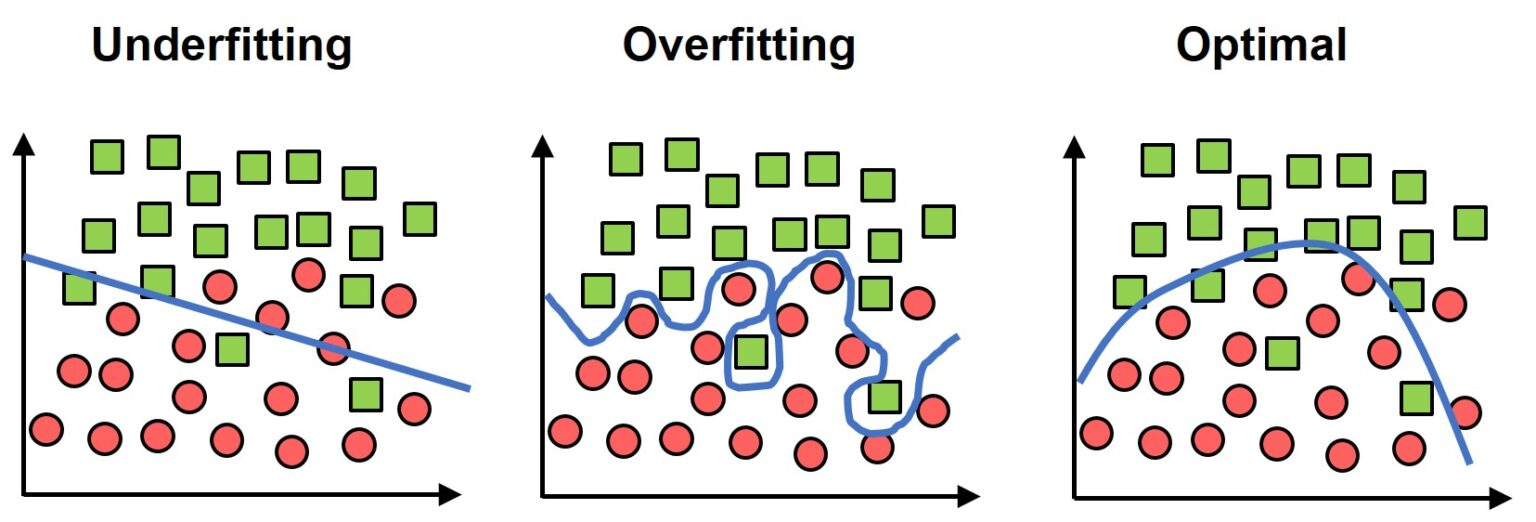
\includegraphics[width=0.8\textwidth]{images/011Fundamentals/overfitting.jpg}
    \caption{Underfitting, Overfitting and Optimal at Deep Learning Trainings. \cite{overfitting_pic} }
    \label{fig:overfitting}
\end{figure}


A key problem in training deep neural networks is overfitting (see Fig. \ref{fig:overfitting}). In this case, the model adapts too strongly to the training data: it achieves high accuracy there, while performance on independent test data decreases significantly. The opposite phenomenon is underfitting, in which the underlying data structure is not sufficiently captured and the model consequently delivers inadequate results in both the training and test data sets. The goal is therefore to develop an optimal model that adequately learns the relevant patterns of the training data and at the same time exhibits a high degree of generalisation ability with respect to unknown data \cite{overfitting_pic}.\\
The high number of parameters in deep networks increases the likelihood that a model will ‘memorise’ the training data excessively and thus lose its ability to make reliable predictions on new test data. Overfitting can be reduced by various regularisation techniques, including weight decay, batch normalisation and dropout. Another option is data augmentation, in which the training dataset is artificially enlarged to improve generalisation ability. Similarly, data corruption – the deliberate inclusion of noisy or manipulated data – can increase the robustness of the model. Finally, there are methods that specifically penalise overly confident predictions, thus also acting as regularisation \cite{Alzubaidi2021}.

In summary, deep learning offers a powerful approach to automated feature extraction and classification that is characterised by flexibility, robustness and high scalability. At the same time, challenges such as the vanishing gradient problem, exploding gradients and overfitting are key areas of research for which new solutions are continuously being developed \cite{Alzubaidi2021}.
 








\section{One Stage and Two Stage Detectors}

The localisation and detection of objects in images can basically be achieved using two approaches: one-stage detectors and two-stage detectors \cite{Soviany2018}.

Two-stage detectors, such as \Acrfull{R-CNN} \cite{ren2016} or Mask \acrshort{R-CNN} \cite{he2018}, consist of two consecutive processing steps. In the first stage, an \Acrfull{RPN} is used to identify potentially relevant image areas. These suggestions are then further processed in the second stage for object classification and bounding box regression. Two-stage approaches generally achieve very high accuracy values, but are more computationally intensive and characterised by lower processing speeds \cite{Soviany2018}.

In contrast, one-stage detectors such as \Acrfull{YOLO} \cite{redmon2016} or \Acrfull{SSD} \cite{Liu_2016} treat object detection as a direct regression problem. The input image is processed in a single step, predicting both class memberships and bounding box coordinates. This approach enables significantly higher processing speeds but generally achieves lower accuracy rates compared to two-stage detectors \cite{Soviany2018}.



\section{Milestones and Historical Development of YOLO Architectures}

\acrfull{YOLO} is a one-stage detector that was first published in the YOLOv1 version by Redmon et al. (2016) \cite{redmon2016}. This approach represented a novel way of object detection, as it combined accuracy and speed by processing images in a single-stage network architecture. YOLOv1 thus laid the foundation for real-time applications in image processing and became the standard for subsequent developments \cite{Sapkota2025}.

Building on YOLOv1, YOLOv2 and YOLO9000 \cite{Li2018,Nakahara2018} improved the resolution at which the model operated and expanded object detection to more than 9,000 categories. YOLOv3 introduced multi-scale predictions and a deeper network architecture to optimise the detection of small objects in particular \cite{Kim2018}.

YOLOv4 spawned several major variants. The standard version, YOLOv4-CSP, integrated \acrlongpl{CSPN} to improve performance, while YOLOv4x-mish utilised the Mish activation function to increase accuracy while maintaining efficiency \cite{Nepal2022,Sozzi2022,Mohod2023}.

In 2020, Ultralytics developed YOLOv5, which impressed with its improved user-friendliness and performance. Five main variants were introduced, covering different areas of application – from resource-saving speed to maximum accuracy on powerful hardware \cite{Sapkota2025,ultralyics_2020}. Subsequent versions YOLOv5 to YOLOv11 built on this foundation, focusing on improved scalability, reduced computational requirements, and optimised real-time performance metrics.

YOLOv6, introduced in 2022 by a team from a Chinese e-commerce platform operator \cite{li2022}, featured a novel backbone and neck architecture. In addition, advanced training techniques such as \acrfull{AAT} and self-distillation were implemented \cite{Sapkota2025,li2022}. YOLOv7 \cite{wang2022,Wang2023} introduced further innovations, including trainable bag of freebies, i.e. optimisations to increase accuracy without additional inference costs, as well as dynamic label assignments \cite{wang2022,Wang2023,Sapkota2025}.

YOLOv8, released in 2023 by Ultralytics \cite{ultralyics_2023}, featured a more efficient architecture, improved training techniques, and expanded support for large datasets \cite{Sapkota2025,ultralyics_2023}. YOLOv9 \cite{wang2024_sapkota} integrated \acrfull{PGI} for more efficient use of deeper networks and introduced the lightweight network architecture \acrfull{GELAN}, which is based on gradient path planning and, in combination with \acrshort{PGI}, achieves particularly good results on resource-efficient models \cite {Sapkota2025,wang2024_sapkota}. This version is used in this work.

YOLOv10, developed in 2023 by Chinese scientists \cite{wang2024}, presented a novel approach to real-time object detection. By eliminating \acrfull{NMS} and optimising key model components, it overcame the limitations of earlier YOLO versions, resulting in significant improvements in efficiency and performance \cite{wang2024}. YOLOv11 further improved the backbone and neck architecture, optimising feature extraction and achieving a balance between precision and computational efficiency \cite{Sapkota2025,ultralyics_yolov11}.

Finally, YOLOv12 utilises an attention-centred approach and implements \acrfull{AA2} and \acrfull{R-ELAN} to further improve feature processing \cite{tian2025,Sapkota2025}.


\section{Evaluation Metrics}
\subsection{K Fold Cross Validation}

The \acrfull{KFC} is one of the most commonly used methods for model selection and error estimation in classification tasks. In this technique, the data set is divided into $k$ equal subsets. Iteratively, $k-1$ of these subsets are used to train the model, while the remaining subset is used to evaluate the model performance \cite{Anguita2012}. In practice, $k$ is often set to 5 or 10, as estimates with these values are characterised by neither high bias nor very high variance \cite{Nti2021}.
 
In addition, K-fold cross-validation enables the data set to be divided into training, validation and test sets in a structured manner. It is important to ensure that the distribution of class objects and the number of images in the individual folds is largely homogeneous. Overlaps of images between different folds must be avoided, as the model otherwise runs the risk of overfitting if identical images are contained in the training, validation and test data sets.



\subsection{Intersection over Union (IoU)}

\begin{figure}[h]
    \centering
    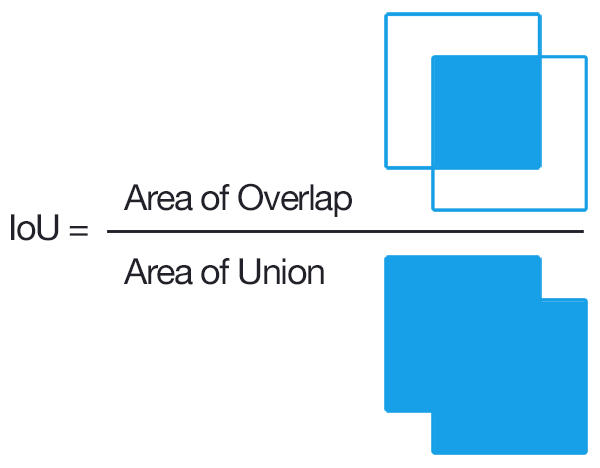
\includegraphics[width=0.4\textwidth]{images/011Fundamentals/IoU.png}
    \caption{Graphical Visualiziation for IoU. \cite{iou_pic}}
    \label{fig:IoU}
\end{figure}

The \acrfull{IoU} (for a graphical explanation, see Fig.\ref{fig:IoU}), also known as the Jaccard index, is the most commonly used metric for comparing the similarity of two arbitrary shapes. It encodes the shape characteristics of the objects to be compared, such as the height, width and position of two \acrfull{BB}, into an area property and uses this to calculate a normalised measure that refers to the compared areas or volumes (see Fig. \ref{fig:IoU}). This property makes the \acrshort{IoU} independent of the size of the object under consideration \cite{Rezatofighi2019}.

Due to this independence, a large number of performance measures are based on segmentation \cite{Ramirez2019,cordts2016,Zhou2017,lin2015}, object detection \cite{lin2015,Everingham2010}, and object tracking \cite{Kristan2016,lealtaixé2015} are based on the \acrshort{IoU}. One of the two \acrshort{BB} corresponds to the \acrfull{GT}, i.e. the correctly labelled and localised object, while the second \acrshort{BB} represents the model's predicted localisation of the object. The agreement (\acrshort{IoU}) calculated on this basis, in which the overlap area of the two bounding boxes is divided by the total area covered by both, enables a precise evaluation of the accuracy of deep learning models.
\begin{definition}[Intersection over Union]
    Let $B_t$ be the set of image pixels covered by a \acrlong{GT} Bounding Box for a class $k$, 
    and $B_p$ be the set of image pixels covered by a predicted Bounding Box for the same class. 
    Then the IoU is calculated as follows:

    \begin{equation}
    \text{IoU}_k =
    \begin{cases}
        \dfrac{|B_t \cap B_p|}{|B_t \cup B_p|}, & \text{if } |B_t \cup B_p| > 0, \\[6pt]
        0, & \text{otherwise.}
    \end{cases}
    \end{equation}

\end{definition}








\subsection{Mean Average Precision (mAP)}

The \acrlong{IoU} is closely related to the \acrfull{mAP}, but is not identical. While the \acrshort{IoU} measures the accuracy of a single predicted \acrshort{BB}, the \acrshort{mAP} is a more comprehensive metric that evaluates the performance of a model across all objects and classes in a dataset \cite {ultralyics_iou}.

The concepts of precision and recall are used to calculate \acrshort{mAP}. Precision describes the proportion of detections classified as positive by the model that are actually correct, while recall indicates the proportion of objects that are actually present and have been correctly detected. Based on these values, a \acrfull{PRC} (see Def. \ref{Def:IPRC}) can be created, with precision plotted on the Y-axis and recall on the X-axis \cite{Goodfellow-et-al-2016}. Object detectors provide a confidence value for each bounding box, which reflects the model's certainty regarding the prediction. Predictions whose confidence is below a specified threshold can be discarded.
 

\begin{definition}[Interpolated Precision-Recall Curve]
\label{Def:IPRC}
Let $P(r)$ be the value of precision at recall value $r$. 
The interpolation of the precision-recall curve is then given by $P_{int}$.

\begin{equation}
P_{int}(r) = \max_{r \leq y} P(y)
\end{equation}
\end{definition}


The \acrshort{PRC} can be created for all possible confidence thresholds, allowing the average precision to be calculated as the area under the curve. The model is then evaluated using the \acrfull{mAP} (see Form. \ref{form:mAP}), which is calculated as the mean value of the \acrfull{AP} (see Form. \ref{form:AP}) across all classes (see Def. \ref{Def:mAP})\cite{Rainio2024}. Different accuracy requirements can be set for the matching of the bounding boxes, for example by using IoU thresholds of 0.5 or a range from 0.5 to 0.95. The latter corresponds to the mean value of \acrshort{mAP}@0.5, \acrshort{mAP}@0.55 to \acrshort{mAP}@0.95. This stricter metric requires greater overlap between \acrshort{GT} and prediction and is particularly suitable when the predicted positions of the bounding boxes must be very precise \cite{Rainio2024}.


\begin{definition}[Mean Average Precision]
\label{Def:mAP}
Let $C$ be the set of classes with $c \in C$, and $P_{int}(r)$ be the interpolated precision-recall curve. 
The Average Precision (AP) and the mean Average Precision (mAP) are then defined as follows:

\begin{equation}
\label{form:AP}
AP_c = \int_0^1 P_{int}(r)\,dr
\end{equation}

\begin{equation}
\label{form:mAP}
mAP = \frac{1}{|C|} \sum_c AP_c
\end{equation}
\end{definition}





